\documentclass[12pt,a4paper]{report}

\usepackage[utf8]{inputenc}
\usepackage[czech]{babel}
\languageattribute{czech}{split}

\usepackage[T1]{fontenc}
\usepackage{lmodern} %ceske fonty

\usepackage{url}

\usepackage{geometry}
\usepackage{xcolor}
\usepackage{amsmath}
\usepackage[some]{background}

\usepackage{graphicx}

\usepackage{framed}
\usepackage{footmisc}

%TODO select color coresponding to logo
\definecolor{titlepagecolor}{cmyk}{1,.60,0,.40}

\backgroundsetup{
scale=1,
angle=0,
opacity=1,
contents={
\begin{tikzpicture}[remember picture,overlay]
  \path [fill=titlepagecolor] (current page.west)rectangle (current page.north east); 
  \draw [color=white, very thick] (5,0)--(5,0.5\paperheight);
 \end{tikzpicture}}
}

\DeclareFixedFont{\bigsf}{T1}{phv}{b}{n}{1.5cm}

\usepackage[unicode,colorlinks=true]{hyperref}
\hypersetup{pdftitle=TextAn - user documentation}
\hypersetup{pdfauthor={Petr Fanta, Adam Huječek}}
\hypersetup{linkcolor=black, citecolor=black, urlcolor=black, filecolor=black}

\makeatletter
\def\@makechapterhead#1{
  {\parindent \z@ \raggedright \normalfont
   \Huge\bfseries \thechapter. #1
   \par\nobreak
   \vskip 20\p@
}}
\def\@makeschapterhead#1{
  {\parindent \z@ \raggedright \normalfont
   \Huge\bfseries #1
   \par\nobreak
   \vskip 20\p@
}}
\makeatother

\def\chapwithtoc#1{
\chapter*{#1}
\addcontentsline{toc}{chapter}{#1}
}

\newcommand{\textan}{\emph{TextAn}}

%\setkeys{Gin}{resolution=96}

\begin{document}

%TODO better titlepage
\begin{titlepage}
\BgThispage

\newgeometry{left=2cm,right=6cm,bottom=2cm}
\vspace*{0.3\textheight}
\noindent
\textcolor{white}{\bigsf TextAn}

\vspace*{1cm}
\noindent
\textcolor{white}{\Huge\textbf{\textsf{Velmi stručný úvod}}}

\vspace*{2cm}\par
\noindent
\begin{minipage}{0.35\linewidth}
\textbf{Authors}

Petr Fanta\\
Adam Huječek\vspace{40pt} \\
\textbf{Version} \\
0.1.1\vspace{40pt} \\
\textbf{Date} \\
\today \\
\end{minipage}

%TODO add logo

\end{titlepage}
\restoregeometry

\pagenumbering{roman}
\tableofcontents

%\chapter*{Intro}
%\addcontentsline{toc}{chapter}{Intro}


\chapter{Klient}
\pagenumbering{arabic}

\section{Instalace}

\subsection{Prerekvizity}
Klient \textan u vyžaduje pro spuštění prostředí \emph{Java 8}, konkrétně JRE\footnote{Doporučujeme použití JRE od firmy \emph{Oracle} dostupné na: http://\url{www.oracle.com/technetwork/java/javase/downloads/index.html}}.

\subsection{Instalace}
K instalaci klienta stačí rozbalit archiv obsahující .jar soubor a spouštěcí skripty pro jednotlivé operační systémy\footnote{run.bat pro operační systém Windows a run.sh pro linuxové operační systémy.\label{runscript_note}} do libovolného adresáře.

\subsection{Konfigurace}
Jestliže se klient nemá připojovat na výchozí server \textan u, je třeba provést jeho konfiguraci. Ta se defaultně nachází v souboru \emph{TextAn.properties}\footnote{popis formátu .properties souborů např. zde: http://en.wikipedia.org/wiki/.properties} v adresáři s .jar souborem klienta. Stačí otevřít tento soubor v textovém editoru (případně ho předtím vytvořit) a přidat následující řádky s URL cílového serveru místo adres serveru výchozího:
\begin{framed}
\noindent
\#url of the document processor\\
url.document=http://textan.ms.mff.cuni.cz:9500/soap/document\\
\#url of the document processor wsdl\\
url.document.wsdl=http://textan.ms.mff.cuni.cz:9500/soap/document?wsdl\\
\#url of the data provider\\
url.data=http://textan.ms.mff.cuni.cz:9500/soap/data\\
\#url of the data provider\\
url.data.wsdl=http://textan.ms.mff.cuni.cz:9500/soap/data?wsdl
\end{framed}

\subsection{Spuštění}
Jar soubor z instalačního archivu je spustitelný, ale přesto doporučujeme ke spouštění používat přiložené skripty pro příslušný operační systém\footref{runscript_note}.

%\section{Kompilace}
%TODO

\section{Použití}

\subsection{První spuštění}
Při prvním spuštění klienta je uživatel nejdříve vyzván k zadání uživatelského jména (viz obr. \ref{fig:First}), které je v systému využíváno k identifikaci uživatelů. Toto jméno se ukládá a při dalším spuštění aplikace již není znovu vyžadováno, ale lze ho později změnit v nastavení (viz sekce \ref{sec:Nastaveni}).

Klient požaduje validní uživatelské jméno, tedy neprázdné a neobsahující pouze bílé znaky. Pokud uživatel zadá jméno nevalidní, je na tuto skutečnost upozorněn a může jméno zadat znovu, případně se aplikace ukončí.

\begin{figure}[!htb]
	\centering
	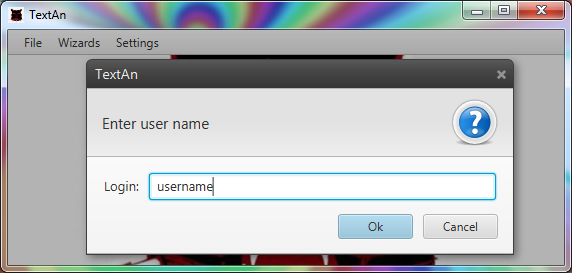
\includegraphics[width=\textwidth]{first}
	\caption{První obrazovka klienta při prvním spuštění.}
	\label{fig:First}
\end{figure}

\subsection{Popis prostředí}
Základní prostředí v této verzi \textan u je velice jednoduché, skládá se z prostoru pro vnitřní okna a hlavního menu, které obsahuje rozbalovací položky, jež umožňují změnu nastavení programu a spouštění průvodců.

%TODO OBRAZEK S NABIDKAMA / PRAZDNE PROSTREDI

\subsection{Nastavení}
\label{sec:Nastaveni}
Pomocí rozbalovací položky \emph{Nastavení} v hlavním menu si uživatel může přizpůsobit prostředí programu. Dále jsou popsané jednotlivé možnosti nastavení.

\paragraph{Samostatná okna.} Při označení této možnosti budou použita samostatná systémová okna místo oken vložených do hlavního okna klienta. 

\paragraph{Hypergrafy.} Tato volba v nastavení ovlivňuje způsob, jakým budou vykreslovány hyperhrany\footnote{Hyperhrana je hrana v hypergrafu. Jedná se o zobecnění pojmu graf. Rozdíl je v tom, že hrany hypergrafu (hyperhrany) mohou spojovat libovolný počet vrcholů, zatímco u grafu spojují hrany vždy dva vrcholy.} v grafech (viz obrázek \ref{fig:Grafy}). Výchozí způsob vykreslování hyperhran je převod hypergrafu na graf pomocí přidání pomocného vrcholu čtvercového tvaru. Při zaškrtnutí této volby budou hrany znázorněny pomocí pozadí grafu.

\begin{figure}[!htb]
	\centering
	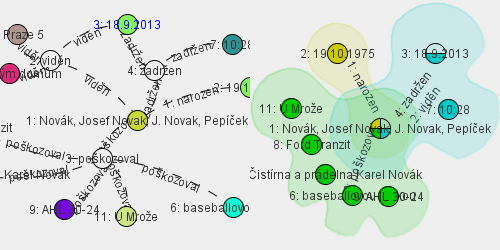
\includegraphics[width=\textwidth]{grafy}
	\caption{Porovnání zobrazení grafů. Výchozí zobrazení je vlevo.}
	\label{fig:Grafy}
\end{figure}

\paragraph{Vymazávat filtry.}
Volba určuje, zda se bude zachovávat hodnota filtrů po zavření okna, které prochází záznamy uložené v databázi.

\paragraph{Lokalizace.}
Přizpůsobí prostředí programu pro daný jazyk. V základní verzi \textan u jsou dostupná česká a anglická lokalizace, která je výchozí. Změna jazyka se projeví až po restartování aplikace.

\paragraph{Vzdálenost v grafech.}
Vzdálenost v grafech určuje výchozí maximální délku cesty v grafu od středového vrcholu. 

\paragraph{Login.}
Tato volba umožňuje změnu aktuálního uživatele. Změna se projeví pouze u nově započatých akcí. Doporučujeme proto následný restart programu.

\subsection{Zpracování dokumentu}
Ke zpracování dokumentů slouží průvodce \emph{Zpráva} dostupný v hlavním menu v sekci \emph{Průvodci}. Při zpracování dokumentu musí uživatel projít postupně fázemi, které obsahují jednotlivé činnosti při zpracování dokumentu. Tyto fáze jsou:

\paragraph{Načtení.}
Umožňuje výběr zdroje dokumentů. Možné zdroje\footnote{V současné verzi \textan u je dostupná pouze možnost \emph{Prázdná správa}} jsou databáze systému (uložené nezpracované dokumenty), textový soubor, prázdná zpráva, či uložená rozpracovaná zpráva. Po výběru zdroje zprávy se uživatel dostane do jedné z následujících fází zpracování dokumentu, typicky do fáze \emph{Editace textu}.

\paragraph{Editace textu.}
V této fázi má uživatel možnost zadat, či změnit text dokumentu. Po této fázi následuje fáze \emph{Editace entit}.

\paragraph{Editace entit.}
Před vstupem do této fáze se systém pokusí rozpoznat pojmenované entity v dokumentu. Rozpoznané entity jsou označeny pomocí různých barev písma. Tyto barvy jsou určeny podle typu entit, jinak řečeno entity stejného typu entit mají stejnou barvu (viz obrázek \ref{fig:Entity}). Typ entity je možné zjistit najetím kurzorem myši na text určující entitu. Rozsah entity je znázorněn pomocí podtržení textu.

\begin{figure}[!htb]
	\centering
	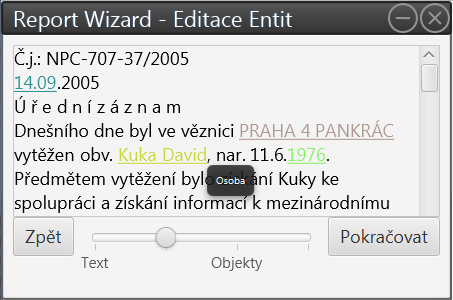
\includegraphics[width=\textwidth]{entity}
	\caption{Příklad rozpoznaných entit s typem entity.}
	\label{fig:Entity}
\end{figure}

Uživatel může měnit a přidávat entity pomocí výběru textu myší a následného výběru typu entity ze zobrazené nabídky. Jedna entita se nemůže skládat z více oddělených částí a entity se nemohou překrývat.

Na tuto fázi zpracování navazuje fáze \emph{Editace objektů}.

\paragraph{Editace objektů}
Cílem této fáze je přiřazení entit k reálným objektům. Před vstupem do této fáze se systém pokusí sám přiřadit\footnote{V současné verzi \textan u tato funkčnost není implementována, proto je přiřazen jakýkoliv objekt stejného typu jako je entita.} k entitám objekty, které jsou v databázi, nebo najít objekty, které by daná entita mohla reprezentovat. Pokud entita nemá přiřazený žádný objekt, je její text zvýrazněn pomocí oranžového pozadí.

Pro zjištění přiřazeného objektu či typu entity opět stačí najet myší na text objektu. Přiřazení objektu k entitě je možné provést pomocí kliknutí levým tlačítkem myši na text entity a následně zobrazené nabídky (viz obrázek \ref{fig:Objekty}). Pomocí kliknutí pravým tlačítkem myši na text entity s přiřazeným objektem lze získat více informací o přiřazeném objektu, například zobrazit graf s okolím daného objektu.

\begin{figure}[!htb]
	\centering
	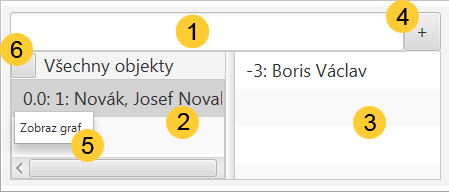
\includegraphics[width=\textwidth]{objekty}
	\caption{Nabídka pro výběr objektu. 1) Filtrování objektů z databáze, 2) Seznam doporučených objektů, při zaškrtnuté 6) seznam všech objektů daného typu v databázi, 3) Seznam nových objektů vytvořených během editace a stejného typu, jako má entita, 4) Tlačítko pro vytvoření nového objektu, 5) Nabídka pro získání informací o objektu z databáze.}
	\label{fig:Objekty}
\end{figure}

Po přiřazení objektu všem entitám je možné přejít do poslední povinné fáze zpracování dokumentu, a to \emph{Editace vztahů}.

\paragraph{Editace vztahů}
Poslední fází zpracování dokumentu je označení vztahů mezi objekty v dokumentu. Vztahy mohou být dvou typů: s kotvou\footnote{Kotva je nějaké slovo, či slovní spojení v textu, které určuje vztah, typicky přísudek ve větě.} v textu a bez kotvy.

Vztah s kotvou je možné vytvořit pomocí výběru kotvy v textu pomocí myši a následného výběru typu vztahu. Prázdný vztah s danou kotvou a typem je poté přidán do seznamu vztahů. Prázdný vztah bez kotvy lze přidat do seznamu pomocí tlačítka pod seznamem vztahů.

Pro přidání objektů do vztahů je nutné nejprve vybrat vztah v seznamu vztahů a následně se objekty přidávají pomocí seznamu objektů ve vztahu.

Po dokončení editace vztahů je možné zpracovaný dokument uložit do databáze systému.

\begin{figure}[!htb]
	\centering
	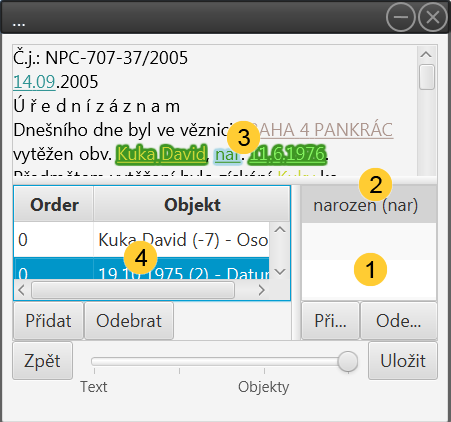
\includegraphics[width=\textwidth]{vztahy}
	\caption{Okno pro výběr vztahů. 1) Seznam vztahů, 2) Vztah s kotvou, 3) Zobrazení vztahu v textu, 4) Seznam objektů ve vztahu.}	
	\label{fig:Vztahy}
\end{figure}

\paragraph{}
Během editace dokumentu je možné se vracet k předchozím fázím zpracování. Pokud jsou však po návratu provedeny nějaké změny, všechny následující fáze jsou zahozeny.

\subsection{Procházení objektů}
Procházení objektů v databázi možné pomocí průvodce \emph{Objekty}, který je dostupný z hlavního menu. Průvodce obsahuje výpis objektů, které je možné filtrovat podle typů a aliasů objektů.

Pomocí pravého tlačítka myši je možné zobrazit podrobnější informace o objektu, například graf s okolím objektu.

\subsection{Manipulace s grafy}
Okno s grafem je možné zobrazit z mnoha míst v programu, typicky kliknutím pravým tlačítkem na nějakou reprezentaci objektu.

V horní části okna s grafem se nachází lišta umožnující jednak změnu velikosti okolí středového vrcholu, jednak výběr nástrojů pro manipulaci s grafem. Nástroj \emph{Transformace} složí k transformaci grafu jako celku, například posunutí celého plátna s grafem, či rotace grafu pomocí stisku \emph{CTRL} a tažením myší. Naopak nástroj \emph{Výběr} slouží k manipulaci s jednotlivými vrcholy a hranami. Graf je také možné přibližovat a oddalovat pomocí kolečka myši.

Na vrcholy reprezentující objekty lze opět kliknout pomocí pravého tlačítka myši a získat další informace o objektu.

%\subsection{Pokročilé nastavení}



\end{document}